\documentclass[12pt]{article}

\usepackage{amsmath, amssymb}
\usepackage[margin=1in]{geometry}
\usepackage{helvet}
\usepackage{tikz}
% \usepackage{figure}
\renewcommand{\familydefault}{\sfdefault}

\begin{document}
\def\assignment{Homework 07}

\pagenumbering{gobble}
\noindent{\large COSC 4200 \hfill Name: \underline{Jacob Tuttle} \\ Computability \& Complexity}
\begin{center}
    {\Large \assignment} \\ \textbf{\today}
\end{center}

\begin{enumerate}
    \item \begin{enumerate}
        \item A DFA can be constructed through product construction to show that $A - B$ is regular. Let Q be all states $(a_i, b_j)$ where $(a_i, b_j) \in A \times B$. Then, let $\delta^*$ be the extended transition function created in the construction. Finally, include the pair $(a_i, b_j)$ in $F$ if $a_i \in F_A$ and $b_j \in F_B$. In this way, we define a DFA that accepts $A - B$ demonstrating it is regular.

        \item Using the above demonstration that $A - B$ is regular, let us next construct the DFA corresponding to $B - A$. Then, since regular languages are closed under union, we know that $A \Delta B$ is regular.

    \end{enumerate}
    \item \begin{enumerate}
        \item This NFA will check that a 1 is present first, a 0 is present in the last position, and then allow anything else to be read in between that.
            \begin{center}
            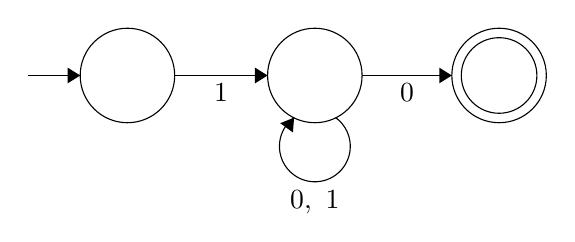
\begin{tikzpicture}[scale=0.2]
            \tikzstyle{every node}+=[inner sep=0pt]
            \draw [black] (10.2,-8.5) circle (3);
            \draw [black] (22.1,-8.5) circle (3);
            \draw [black] (33.8,-8.5) circle (3);
            \draw [black] (33.8,-8.5) circle (2.4);
            \draw [black] (3.9,-8.5) -- (7.2,-8.5);
            \fill [black] (7.2,-8.5) -- (6.4,-8) -- (6.4,-9);
            \draw [black] (13.2,-8.5) -- (19.1,-8.5);
            \fill [black] (19.1,-8.5) -- (18.3,-8) -- (18.3,-9);
            \draw (16.15,-9) node [below] {$1$};
            \draw [black] (25.1,-8.5) -- (30.8,-8.5);
            \fill [black] (30.8,-8.5) -- (30,-8) -- (30,-9);
            \draw (27.95,-9) node [below] {$0$};
            \draw [black] (23.423,-11.18) arc (54:-234:2.25);
            \draw (22.1,-15.75) node [below] {$0,\mbox{ }1$};
            \fill [black] (20.78,-11.18) -- (19.9,-11.53) -- (20.71,-12.12);
            \end{tikzpicture}
            \end{center}

        \item This will allow any beginning to the string, and as soon as a 101 or 11 is present at the end of the string, the NFA will escape to the success state.
            \begin{center}
            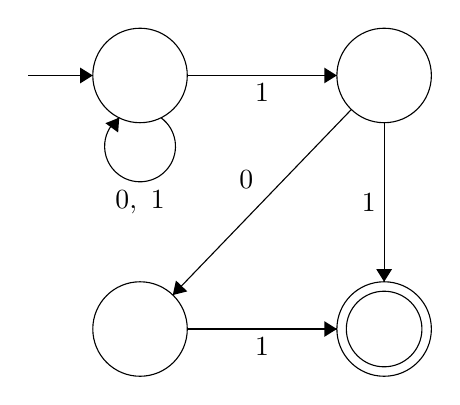
\begin{tikzpicture}[scale=0.2]
            \tikzstyle{every node}+=[inner sep=0pt]
            \draw [black] (9.1,-7.8) circle (3);
            \draw [black] (24.6,-7.8) circle (3);
            \draw [black] (9.1,-23.9) circle (3);
            \draw [black] (24.6,-23.9) circle (3);
            \draw [black] (24.6,-23.9) circle (2.4);
            \draw [black] (2,-7.8) -- (6.1,-7.8);
            \fill [black] (6.1,-7.8) -- (5.3,-7.3) -- (5.3,-8.3);
            \draw [black] (12.1,-7.8) -- (21.6,-7.8);
            \fill [black] (21.6,-7.8) -- (20.8,-7.3) -- (20.8,-8.3);
            \draw (16.85,-8.3) node [below] {$1$};
            \draw [black] (10.423,-10.48) arc (54:-234:2.25);
            \draw (9.1,-15.05) node [below] {$0,\mbox{ }1$};
            \fill [black] (7.78,-10.48) -- (6.9,-10.83) -- (7.71,-11.42);
            \draw [black] (22.52,-9.96) -- (11.18,-21.74);
            \fill [black] (11.18,-21.74) -- (12.1,-21.51) -- (11.38,-20.82);
            \draw (16.32,-14.38) node [left] {$0$};
            \draw [black] (12.1,-23.9) -- (21.6,-23.9);
            \fill [black] (21.6,-23.9) -- (20.8,-23.4) -- (20.8,-24.4);
            \draw (16.85,-24.4) node [below] {$1$};
            \draw [black] (24.6,-10.8) -- (24.6,-20.9);
            \fill [black] (24.6,-20.9) -- (25.1,-20.1) -- (24.1,-20.1);
            \draw (24.1,-15.85) node [left] {$1$};
            \end{tikzpicture}
            \end{center}

        \item This NFA provides free paths for constructions where any of $i, j, k \leq 1$. But, an unacceptable construction would be unnable to make it to the final state because characters would be unread upon reaching the final accessible state and it would then fail.
            \begin{center}
            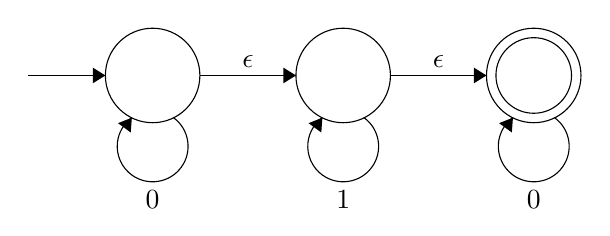
\begin{tikzpicture}[scale=0.2]
            \tikzstyle{every node}+=[inner sep=0pt]
            \draw [black] (9,-6.7) circle (3);
            \draw [black] (21.1,-6.7) circle (3);
            \draw [black] (33.2,-6.7) circle (3);
            \draw [black] (33.2,-6.7) circle (2.4);
            \draw [black] (24.1,-6.7) -- (30.2,-6.7);
            \fill [black] (30.2,-6.7) -- (29.4,-6.2) -- (29.4,-7.2);
            \draw (27.15,-6.2) node [above] {$\epsilon$};
            \draw [black] (12,-6.7) -- (18.1,-6.7);
            \fill [black] (18.1,-6.7) -- (17.3,-6.2) -- (17.3,-7.2);
            \draw (15.05,-6.2) node [above] {$\epsilon$};
            \draw [black] (1.1,-6.7) -- (6,-6.7);
            \fill [black] (6,-6.7) -- (5.2,-6.2) -- (5.2,-7.2);
            \draw [black] (10.323,-9.38) arc (54:-234:2.25);
            \draw (9,-13.95) node [below] {$0$};
            \fill [black] (7.68,-9.38) -- (6.8,-9.73) -- (7.61,-10.32);
            \draw [black] (22.423,-9.38) arc (54:-234:2.25);
            \draw (21.1,-13.95) node [below] {$1$};
            \fill [black] (19.78,-9.38) -- (18.9,-9.73) -- (19.71,-10.32);
            \draw [black] (34.523,-9.38) arc (54:-234:2.25);
            \draw (33.2,-13.95) node [below] {$0$};
            \fill [black] (31.88,-9.38) -- (31,-9.73) -- (31.81,-10.32);
            \end{tikzpicture}
            \end{center}


        \item This NFA will track through states used to determine whether the substring '01010' If the substring is present, then it will exit to a catch-all success state. Otherwise, it will continue moving through failure states.
            \begin{center}
            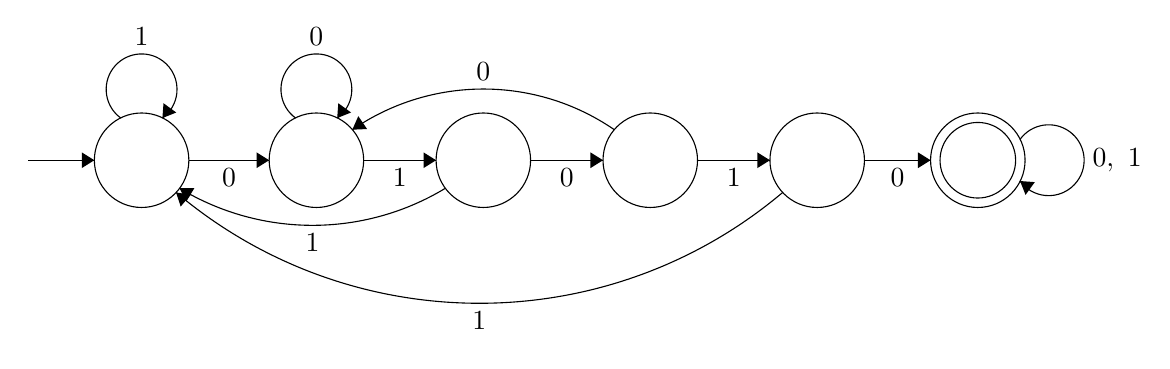
\begin{tikzpicture}[scale=0.2]
            \tikzstyle{every node}+=[inner sep=0pt]
            \draw [black] (9.1,-11.1) circle (3);
            \draw [black] (20.2,-11.1) circle (3);
            \draw [black] (30.8,-11.1) circle (3);
            \draw [black] (41.4,-11.1) circle (3);
            \draw [black] (52,-11.1) circle (3);
            \draw [black] (62.2,-11.1) circle (3);
            \draw [black] (62.2,-11.1) circle (2.4);
            \draw [black] (1.9,-11.1) -- (6.1,-11.1);
            \fill [black] (6.1,-11.1) -- (5.3,-10.6) -- (5.3,-11.6);
            \draw [black] (12.1,-11.1) -- (17.2,-11.1);
            \fill [black] (17.2,-11.1) -- (16.4,-10.6) -- (16.4,-11.6);
            \draw (14.65,-11.6) node [below] {$0$};
            \draw [black] (23.2,-11.1) -- (27.8,-11.1);
            \fill [black] (27.8,-11.1) -- (27,-10.6) -- (27,-11.6);
            \draw (25.5,-11.6) node [below] {$1$};
            \draw [black] (33.8,-11.1) -- (38.4,-11.1);
            \fill [black] (38.4,-11.1) -- (37.6,-10.6) -- (37.6,-11.6);
            \draw (36.1,-11.6) node [below] {$0$};
            \draw [black] (44.4,-11.1) -- (49,-11.1);
            \fill [black] (49,-11.1) -- (48.2,-10.6) -- (48.2,-11.6);
            \draw (46.7,-11.6) node [below] {$1$};
            \draw [black] (55,-11.1) -- (59.2,-11.1);
            \fill [black] (59.2,-11.1) -- (58.4,-10.6) -- (58.4,-11.6);
            \draw (57.1,-11.6) node [below] {$0$};
            \draw [black] (64.88,-9.777) arc (144:-144:2.25);
            \draw (69.45,-11.1) node [right] {$0,\mbox{ }1$};
            \fill [black] (64.88,-12.42) -- (65.23,-13.3) -- (65.82,-12.49);
            \draw [black] (7.777,-8.42) arc (234:-54:2.25);
            \draw (9.1,-3.85) node [above] {$1$};
            \fill [black] (10.42,-8.42) -- (11.3,-8.07) -- (10.49,-7.48);
            \draw [black] (28.39,-12.88) arc (-58.82788:-121.17212:16.306);
            \fill [black] (11.51,-12.88) -- (11.94,-13.72) -- (12.45,-12.87);
            \draw (19.95,-15.73) node [below] {$1$};
            \draw [black] (49.808,-13.146) arc (-49.84655:-130.15345:29.865);
            \fill [black] (11.29,-13.15) -- (11.58,-14.04) -- (12.23,-13.28);
            \draw (30.55,-20.68) node [below] {$1$};
            \draw [black] (22.482,-9.161) arc (124.50183:55.49817:14.685);
            \fill [black] (22.48,-9.16) -- (23.42,-9.12) -- (22.86,-8.3);
            \draw (30.8,-6.08) node [above] {$0$};
            \draw [black] (18.877,-8.42) arc (234:-54:2.25);
            \draw (20.2,-3.85) node [above] {$0$};
            \fill [black] (21.52,-8.42) -- (22.4,-8.07) -- (21.59,-7.48);
            \end{tikzpicture}
            \end{center}

        \item This NFA moves to one of four branches to keep track of the first two characters that are read into the NFA. Then, the NFA will continue looping until it's able to follow a path out to an acceptance state that is the reverse of the first two characters. This NFA representation has 2 less states and 12 less edges.
            \begin{center}
            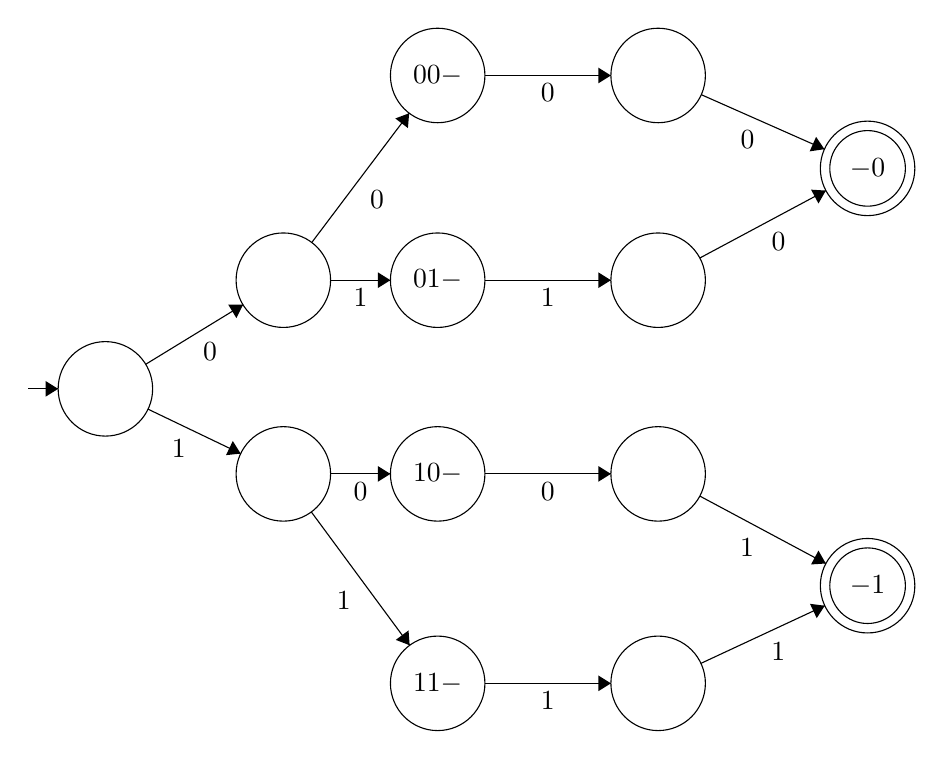
\begin{tikzpicture}[scale=0.2]
            \tikzstyle{every node}+=[inner sep=0pt]
            \draw [black] (5.2,-24.8) circle (3);
            \draw [black] (16.5,-17.9) circle (3);
            \draw [black] (16.5,-30.2) circle (3);
            \draw [black] (26.3,-4.9) circle (3);
            \draw (26.3,-4.9) node {$00-$};
            \draw [black] (26.3,-17.9) circle (3);
            \draw (26.3,-17.9) node {$01-$};
            \draw [black] (26.3,-30.2) circle (3);
            \draw (26.3,-30.2) node {$10-$};
            \draw [black] (26.3,-43.5) circle (3);
            \draw (26.3,-43.5) node {$11-$};
            \draw [black] (40.3,-4.9) circle (3);
            \draw [black] (40.3,-17.9) circle (3);
            \draw [black] (40.3,-30.2) circle (3);
            \draw [black] (40.3,-43.5) circle (3);
            \draw [black] (53.6,-10.8) circle (3);
            \draw (53.6,-10.8) node {$-0$};
            \draw [black] (53.6,-10.8) circle (2.4);
            \draw [black] (53.6,-37.3) circle (3);
            \draw (53.6,-37.3) node {$-1$};
            \draw [black] (53.6,-37.3) circle (2.4);
            \draw [black] (19.5,-17.9) -- (23.3,-17.9);
            \fill [black] (23.3,-17.9) -- (22.5,-17.4) -- (22.5,-18.4);
            \draw (21.4,-18.4) node [below] {$1$};
            \draw [black] (19.5,-30.2) -- (23.3,-30.2);
            \fill [black] (23.3,-30.2) -- (22.5,-29.7) -- (22.5,-30.7);
            \draw (21.4,-30.7) node [below] {$0$};
            \draw [black] (18.31,-15.5) -- (24.49,-7.3);
            \fill [black] (24.49,-7.3) -- (23.61,-7.63) -- (24.41,-8.24);
            \draw (21.98,-12.8) node [right] {$0$};
            \draw [black] (18.28,-32.62) -- (24.52,-41.08);
            \fill [black] (24.52,-41.08) -- (24.45,-40.14) -- (23.64,-40.74);
            \draw (20.82,-38.24) node [left] {$1$};
            \draw [black] (7.76,-23.24) -- (13.94,-19.46);
            \fill [black] (13.94,-19.46) -- (13,-19.45) -- (13.52,-20.31);
            \draw (11.85,-21.85) node [below] {$0$};
            \draw [black] (7.91,-26.09) -- (13.79,-28.91);
            \fill [black] (13.79,-28.91) -- (13.29,-28.11) -- (12.86,-29.01);
            \draw (9.86,-28.01) node [below] {$1$};
            \draw [black] (29.3,-4.9) -- (37.3,-4.9);
            \fill [black] (37.3,-4.9) -- (36.5,-4.4) -- (36.5,-5.4);
            \draw (33.3,-5.4) node [below] {$0$};
            \draw [black] (43.04,-6.12) -- (50.86,-9.58);
            \fill [black] (50.86,-9.58) -- (50.33,-8.8) -- (49.92,-9.72);
            \draw (45.97,-8.36) node [below] {$0$};
            \draw [black] (29.3,-17.9) -- (37.3,-17.9);
            \fill [black] (37.3,-17.9) -- (36.5,-17.4) -- (36.5,-18.4);
            \draw (33.3,-18.4) node [below] {$1$};
            \draw [black] (42.95,-16.49) -- (50.95,-12.21);
            \fill [black] (50.95,-12.21) -- (50.01,-12.15) -- (50.48,-13.03);
            \draw (47.95,-14.85) node [below] {$0$};
            \draw [black] (29.3,-30.2) -- (37.3,-30.2);
            \fill [black] (37.3,-30.2) -- (36.5,-29.7) -- (36.5,-30.7);
            \draw (33.3,-30.7) node [below] {$0$};
            \draw [black] (29.3,-43.5) -- (37.3,-43.5);
            \fill [black] (37.3,-43.5) -- (36.5,-43) -- (36.5,-44);
            \draw (33.3,-44) node [below] {$1$};
            \draw [black] (42.95,-31.61) -- (50.95,-35.89);
            \fill [black] (50.95,-35.89) -- (50.48,-35.07) -- (50.01,-35.95);
            \draw (45.95,-34.25) node [below] {$1$};
            \draw [black] (43.02,-42.23) -- (50.88,-38.57);
            \fill [black] (50.88,-38.57) -- (49.94,-38.45) -- (50.37,-39.36);
            \draw (47.93,-40.91) node [below] {$1$};
            \draw [black] (0.3,-24.8) -- (2.2,-24.8);
            \fill [black] (2.2,-24.8) -- (1.4,-24.3) -- (1.4,-25.3);
            \end{tikzpicture}
            \end{center}

        \item This NFA will jump to one of two branches that keeps track of the first character read. Then, if the last character is different than the first character read, the NFA will jump to an acceptance state.
            \begin{center}
            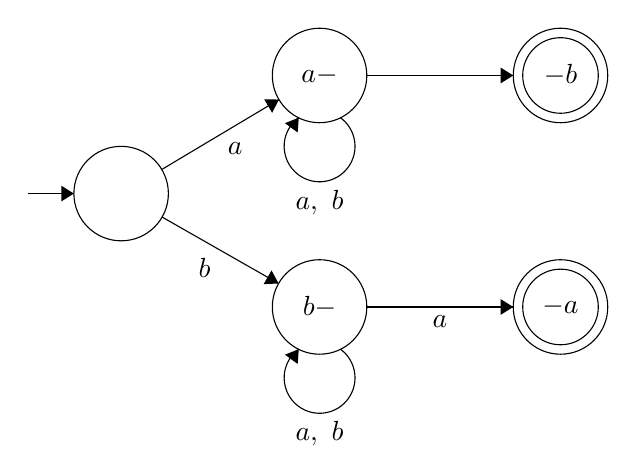
\begin{tikzpicture}[scale=0.2]
            \tikzstyle{every node}+=[inner sep=0pt]
            \draw [black] (8.1,-13.3) circle (3);
            \draw [black] (20.7,-5.8) circle (3);
            \draw (20.7,-5.8) node {$a-$};
            \draw [black] (36,-5.8) circle (3);
            \draw (36,-5.8) node {$-b$};
            \draw [black] (36,-5.8) circle (2.4);
            \draw [black] (20.7,-20.5) circle (3);
            \draw (20.7,-20.5) node {$b-$};
            \draw [black] (36,-20.5) circle (3);
            \draw (36,-20.5) node {$-a$};
            \draw [black] (36,-20.5) circle (2.4);
            \draw [black] (23.7,-20.5) -- (33,-20.5);
            \fill [black] (33,-20.5) -- (32.2,-20) -- (32.2,-21);
            \draw (28.35,-21) node [below] {$a$};
            \draw [black] (23.7,-5.8) -- (33,-5.8);
            \fill [black] (33,-5.8) -- (32.2,-5.3) -- (32.2,-6.3);
            \draw [black] (10.68,-11.77) -- (18.12,-7.33);
            \fill [black] (18.12,-7.33) -- (17.18,-7.31) -- (17.69,-8.17);
            \draw (15.34,-10.05) node [below] {$a$};
            \draw [black] (10.7,-14.79) -- (18.1,-19.01);
            \fill [black] (18.1,-19.01) -- (17.65,-18.18) -- (17.15,-19.05);
            \draw (13.4,-17.4) node [below] {$b$};
            \draw [black] (2.2,-13.3) -- (5.1,-13.3);
            \fill [black] (5.1,-13.3) -- (4.3,-12.8) -- (4.3,-13.8);
            \draw [black] (22.023,-8.48) arc (54:-234:2.25);
            \draw (20.7,-13.05) node [below] {$a,\mbox{ }b$};
            \fill [black] (19.38,-8.48) -- (18.5,-8.83) -- (19.31,-9.42);
            \draw [black] (22.023,-23.18) arc (54:-234:2.25);
            \draw (20.7,-27.75) node [below] {$a,\mbox{ }b$};
            \fill [black] (19.38,-23.18) -- (18.5,-23.53) -- (19.31,-24.12);
            \end{tikzpicture}
            \end{center}

    \end{enumerate}
    \item This NFA will drop into a fail state at any point where two bs are present in a row and moves to the right hand side where acceptance states are present after an aba has been read.
        \begin{center}
        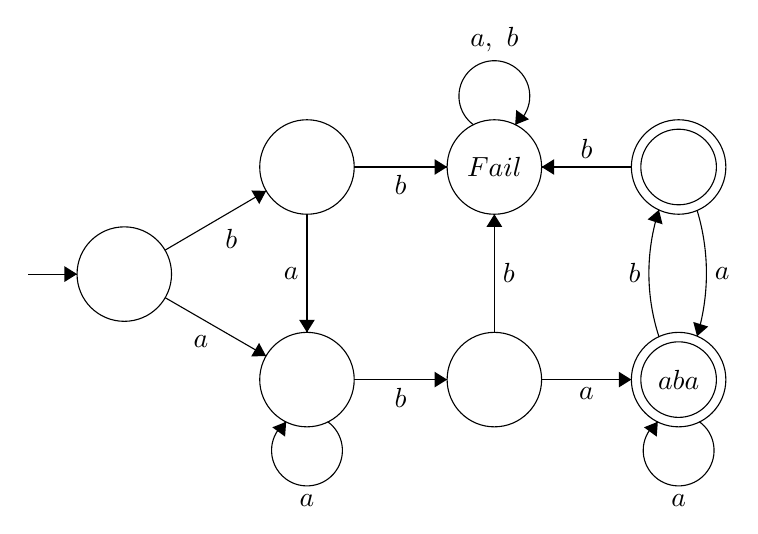
\begin{tikzpicture}[scale=0.2]
        \tikzstyle{every node}+=[inner sep=0pt]
        \draw [black] (30.9,-11.2) circle (3);
        \draw (30.9,-11.2) node {$Fail$};
        \draw [black] (30.9,-24.7) circle (3);
        \draw [black] (42.6,-24.7) circle (3);
        \draw (42.6,-24.7) node {$aba$};
        \draw [black] (42.6,-24.7) circle (2.4);
        \draw [black] (42.6,-11.2) circle (3);
        \draw [black] (42.6,-11.2) circle (2.4);
        \draw [black] (19,-11.2) circle (3);
        \draw [black] (19,-24.7) circle (3);
        \draw [black] (7.4,-18) circle (3);
        \draw [black] (39.6,-11.2) -- (33.9,-11.2);
        \fill [black] (33.9,-11.2) -- (34.7,-11.7) -- (34.7,-10.7);
        \draw (36.75,-10.7) node [above] {$b$};
        \draw [black] (29.577,-8.52) arc (234:-54:2.25);
        \draw (30.9,-3.95) node [above] {$a,\mbox{ }b$};
        \fill [black] (32.22,-8.52) -- (33.1,-8.17) -- (32.29,-7.58);
        \draw [black] (22,-11.2) -- (27.9,-11.2);
        \fill [black] (27.9,-11.2) -- (27.1,-10.7) -- (27.1,-11.7);
        \draw (24.95,-11.7) node [below] {$b$};
        \draw [black] (30.9,-21.7) -- (30.9,-14.2);
        \fill [black] (30.9,-14.2) -- (30.4,-15) -- (31.4,-15);
        \draw (31.4,-17.95) node [right] {$b$};
        \draw [black] (41.352,-21.979) arc (-161.96943:-198.03057:13.017);
        \fill [black] (41.35,-13.92) -- (40.63,-14.53) -- (41.58,-14.84);
        \draw (40.21,-17.95) node [left] {$b$};
        \draw [black] (43.774,-13.954) arc (16.85499:-16.85499:13.781);
        \fill [black] (43.77,-21.95) -- (44.48,-21.33) -- (43.53,-21.04);
        \draw (44.87,-17.95) node [right] {$a$};
        \draw [black] (43.923,-27.38) arc (54:-234:2.25);
        \draw (42.6,-31.95) node [below] {$a$};
        \fill [black] (41.28,-27.38) -- (40.4,-27.73) -- (41.21,-28.32);
        \draw [black] (33.9,-24.7) -- (39.6,-24.7);
        \fill [black] (39.6,-24.7) -- (38.8,-24.2) -- (38.8,-25.2);
        \draw (36.75,-25.2) node [below] {$a$};
        \draw [black] (22,-24.7) -- (27.9,-24.7);
        \fill [black] (27.9,-24.7) -- (27.1,-24.2) -- (27.1,-25.2);
        \draw (24.95,-25.2) node [below] {$b$};
        \draw [black] (19,-14.2) -- (19,-21.7);
        \fill [black] (19,-21.7) -- (19.5,-20.9) -- (18.5,-20.9);
        \draw (18.5,-17.95) node [left] {$a$};
        \draw [black] (9.99,-16.48) -- (16.41,-12.72);
        \fill [black] (16.41,-12.72) -- (15.47,-12.69) -- (15.97,-13.55);
        \draw (14.2,-15.1) node [below] {$b$};
        \draw [black] (10,-19.5) -- (16.4,-23.2);
        \fill [black] (16.4,-23.2) -- (15.96,-22.37) -- (15.46,-23.23);
        \draw (12.26,-21.85) node [below] {$a$};
        \draw [black] (20.323,-27.38) arc (54:-234:2.25);
        \draw (19,-31.95) node [below] {$a$};
        \fill [black] (17.68,-27.38) -- (16.8,-27.73) -- (17.61,-28.32);
        \draw [black] (1.3,-18) -- (4.4,-18);
        \fill [black] (4.4,-18) -- (3.6,-17.5) -- (3.6,-18.5);
        \end{tikzpicture}
        \end{center}

    \item The NFA provided in 2d is already a DFA. Every state has a 0 and 1 transition coming from it, and there are no $\epsilon$ transitions in the machine.
        \begin{center}
        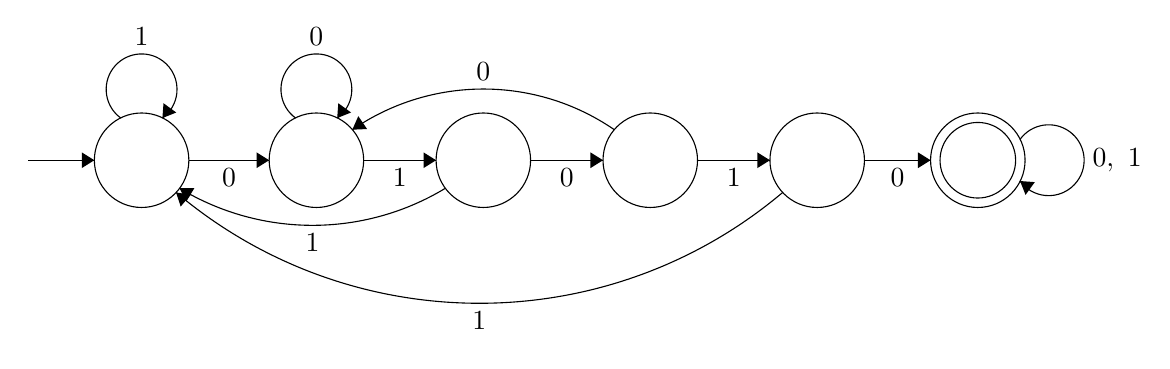
\begin{tikzpicture}[scale=0.2]
        \tikzstyle{every node}+=[inner sep=0pt]
        \draw [black] (9.1,-11.1) circle (3);
        \draw [black] (20.2,-11.1) circle (3);
        \draw [black] (30.8,-11.1) circle (3);
        \draw [black] (41.4,-11.1) circle (3);
        \draw [black] (52,-11.1) circle (3);
        \draw [black] (62.2,-11.1) circle (3);
        \draw [black] (62.2,-11.1) circle (2.4);
        \draw [black] (1.9,-11.1) -- (6.1,-11.1);
        \fill [black] (6.1,-11.1) -- (5.3,-10.6) -- (5.3,-11.6);
        \draw [black] (12.1,-11.1) -- (17.2,-11.1);
        \fill [black] (17.2,-11.1) -- (16.4,-10.6) -- (16.4,-11.6);
        \draw (14.65,-11.6) node [below] {$0$};
        \draw [black] (23.2,-11.1) -- (27.8,-11.1);
        \fill [black] (27.8,-11.1) -- (27,-10.6) -- (27,-11.6);
        \draw (25.5,-11.6) node [below] {$1$};
        \draw [black] (33.8,-11.1) -- (38.4,-11.1);
        \fill [black] (38.4,-11.1) -- (37.6,-10.6) -- (37.6,-11.6);
        \draw (36.1,-11.6) node [below] {$0$};
        \draw [black] (44.4,-11.1) -- (49,-11.1);
        \fill [black] (49,-11.1) -- (48.2,-10.6) -- (48.2,-11.6);
        \draw (46.7,-11.6) node [below] {$1$};
        \draw [black] (55,-11.1) -- (59.2,-11.1);
        \fill [black] (59.2,-11.1) -- (58.4,-10.6) -- (58.4,-11.6);
        \draw (57.1,-11.6) node [below] {$0$};
        \draw [black] (64.88,-9.777) arc (144:-144:2.25);
        \draw (69.45,-11.1) node [right] {$0,\mbox{ }1$};
        \fill [black] (64.88,-12.42) -- (65.23,-13.3) -- (65.82,-12.49);
        \draw [black] (7.777,-8.42) arc (234:-54:2.25);
        \draw (9.1,-3.85) node [above] {$1$};
        \fill [black] (10.42,-8.42) -- (11.3,-8.07) -- (10.49,-7.48);
        \draw [black] (28.39,-12.88) arc (-58.82788:-121.17212:16.306);
        \fill [black] (11.51,-12.88) -- (11.94,-13.72) -- (12.45,-12.87);
        \draw (19.95,-15.73) node [below] {$1$};
        \draw [black] (49.808,-13.146) arc (-49.84655:-130.15345:29.865);
        \fill [black] (11.29,-13.15) -- (11.58,-14.04) -- (12.23,-13.28);
        \draw (30.55,-20.68) node [below] {$1$};
        \draw [black] (22.482,-9.161) arc (124.50183:55.49817:14.685);
        \fill [black] (22.48,-9.16) -- (23.42,-9.12) -- (22.86,-8.3);
        \draw (30.8,-6.08) node [above] {$0$};
        \draw [black] (18.877,-8.42) arc (234:-54:2.25);
        \draw (20.2,-3.85) node [above] {$0$};
        \fill [black] (21.52,-8.42) -- (22.4,-8.07) -- (21.59,-7.48);
        \end{tikzpicture}
        \end{center}

    \item \begin{enumerate}
        \item This language descripes all even length strings.

        \item This language describes all strings of length $\leq$ 3.

        \item This language describes all strings with substring '111' followed somewhere by substring '000.'

        \item This language describes all striongs that start with any number of 0s followed by either 0s or '100' repeatedly.

        \item This language describes all strings made of 0s and 1s.

    \end{enumerate}
    \item \begin{enumerate}
        \item $[(a \cup b)^\star b(a \cup b)^\star b(a \cup b)^\star b(a \cup b)^\star]$

        \item $[(a \cup b)[(a \cup b)b(a \cup b)]^\star[(a \cup b) \cup \epsilon] \cup \epsilon]$

        \item $[b^\star(ab^\star(ab^\star \cup \epsilon) \cup \epsilon)\cup \epsilon]$

        \item $[(aaaaaa)^\star(aaaa \cup [aaa \cup (aa \cup \epsilon)])]$

        \item $[b^\star(ab^\star[ab^\star a (a \cup b)^\star \cup \epsilon]\cup \epsilon)]$

    \end{enumerate}
    \item \begin{enumerate}
        \item This NFA represents the regular expression $[(0 \cup 11)^\star(1 \cup 01)]$
            \begin{center}
            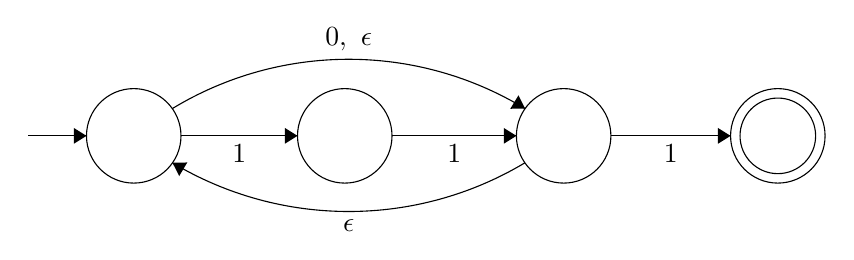
\begin{tikzpicture}[scale=0.2]
            \tikzstyle{every node}+=[inner sep=0pt]
            \draw [black] (8.3,-9.6) circle (3);
            \draw [black] (21.7,-9.6) circle (3);
            \draw [black] (35.6,-9.6) circle (3);
            \draw [black] (49.2,-9.6) circle (3);
            \draw [black] (49.2,-9.6) circle (2.4);
            \draw [black] (1.6,-9.6) -- (5.3,-9.6);
            \fill [black] (5.3,-9.6) -- (4.5,-9.1) -- (4.5,-10.1);
            \draw [black] (11.3,-9.6) -- (18.7,-9.6);
            \fill [black] (18.7,-9.6) -- (17.9,-9.1) -- (17.9,-10.1);
            \draw (15,-10.1) node [below] {$1$};
            \draw [black] (24.7,-9.6) -- (32.6,-9.6);
            \fill [black] (32.6,-9.6) -- (31.8,-9.1) -- (31.8,-10.1);
            \draw (28.65,-10.1) node [below] {$1$};
            \draw [black] (38.6,-9.6) -- (46.2,-9.6);
            \fill [black] (46.2,-9.6) -- (45.4,-9.1) -- (45.4,-10.1);
            \draw (42.4,-10.1) node [below] {$1$};
            \draw [black] (10.748,-7.87) arc (121.25726:58.74274:21.588);
            \fill [black] (33.15,-7.87) -- (32.73,-7.03) -- (32.21,-7.88);
            \draw (21.95,-4.24) node [above] {$0,\mbox{ }\epsilon$};
            \draw [black] (33.14,-11.312) arc (-59.10459:-120.89541:21.792);
            \fill [black] (10.76,-11.31) -- (11.19,-12.15) -- (11.7,-11.29);
            \draw (21.95,-14.9) node [below] {$\epsilon$};
            \end{tikzpicture}
            \end{center}

        \item This NFA represents the regular expression $[(00)^\star 11 \cup 10]^\star$
            \begin{center}
            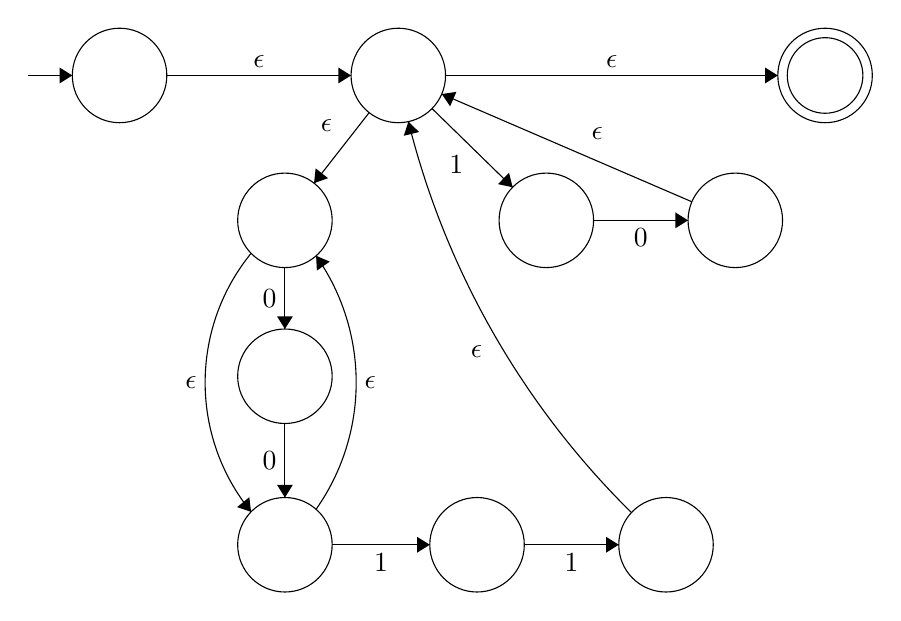
\begin{tikzpicture}[scale=0.2]
            \tikzstyle{every node}+=[inner sep=0pt]
            \draw [black] (9.3,-7.7) circle (3);
            \draw [black] (27,-7.7) circle (3);
            \draw [black] (54.1,-7.7) circle (3);
            \draw [black] (54.1,-7.7) circle (2.4);
            \draw [black] (36.4,-16.9) circle (3);
            \draw [black] (48.4,-16.9) circle (3);
            \draw [black] (19.8,-16.9) circle (3);
            \draw [black] (19.8,-26.8) circle (3);
            \draw [black] (19.8,-37.5) circle (3);
            \draw [black] (32,-37.5) circle (3);
            \draw [black] (44,-37.5) circle (3);
            \draw [black] (3.5,-7.7) -- (6.3,-7.7);
            \fill [black] (6.3,-7.7) -- (5.5,-7.2) -- (5.5,-8.2);
            \draw [black] (12.3,-7.7) -- (24,-7.7);
            \fill [black] (24,-7.7) -- (23.2,-7.2) -- (23.2,-8.2);
            \draw (18.15,-7.2) node [above] {$\epsilon$};
            \draw [black] (30,-7.7) -- (51.1,-7.7);
            \fill [black] (51.1,-7.7) -- (50.3,-7.2) -- (50.3,-8.2);
            \draw (40.55,-7.2) node [above] {$\epsilon$};
            \draw [black] (39.4,-16.9) -- (45.4,-16.9);
            \fill [black] (45.4,-16.9) -- (44.6,-16.4) -- (44.6,-17.4);
            \draw (42.4,-17.4) node [below] {$0$};
            \draw [black] (45.64,-15.72) -- (29.76,-8.88);
            \fill [black] (29.76,-8.88) -- (30.29,-9.66) -- (30.69,-8.74);
            \draw (39.64,-11.78) node [above] {$\epsilon$};
            \draw [black] (29.14,-9.8) -- (34.26,-14.8);
            \fill [black] (34.26,-14.8) -- (34.03,-13.88) -- (33.33,-14.6);
            \draw (30.68,-12.78) node [below] {$1$};
            \draw [black] (25.15,-10.06) -- (21.65,-14.54);
            \fill [black] (21.65,-14.54) -- (22.54,-14.22) -- (21.75,-13.6);
            \draw (22.83,-10.89) node [left] {$\epsilon$};
            \draw [black] (41.805,-35.456) arc (-134.59435:-165.99874:52.803);
            \fill [black] (27.64,-10.63) -- (27.35,-11.53) -- (28.32,-11.29);
            \draw (32.35,-25.24) node [left] {$\epsilon$};
            \draw [black] (19.8,-19.9) -- (19.8,-23.8);
            \fill [black] (19.8,-23.8) -- (20.3,-23) -- (19.3,-23);
            \draw (19.3,-21.85) node [left] {$0$};
            \draw [black] (19.8,-29.8) -- (19.8,-34.5);
            \fill [black] (19.8,-34.5) -- (20.3,-33.7) -- (19.3,-33.7);
            \draw (19.3,-32.15) node [left] {$0$};
            \draw [black] (22.8,-37.5) -- (29,-37.5);
            \fill [black] (29,-37.5) -- (28.2,-37) -- (28.2,-38);
            \draw (25.9,-38) node [below] {$1$};
            \draw [black] (35,-37.5) -- (41,-37.5);
            \fill [black] (41,-37.5) -- (40.2,-37) -- (40.2,-38);
            \draw (38,-38) node [below] {$1$};
            \draw [black] (21.776,-19.15) arc (35.14508:-35.14508:13.985);
            \fill [black] (21.78,-19.15) -- (21.83,-20.09) -- (22.65,-19.52);
            \draw (24.83,-27.2) node [right] {$\epsilon$};
            \draw [black] (17.655,-35.413) arc (-140.82418:-219.17582:13.001);
            \fill [black] (17.65,-35.41) -- (17.54,-34.48) -- (16.76,-35.11);
            \draw (14.23,-27.2) node [left] {$\epsilon$};
            \end{tikzpicture}
            \end{center}

    \end{enumerate}

    \item Constructed through reduction on a DFA representing the states, the regular expression is $[1([0010^\star \cup 1][101^\star 0]^\star 0)^\star ([0010^\star \cup 1][101^\star 0]^\star 11 \cup 01)]\cup 0^\star$

\end{enumerate}
\end{document}
